% 2019 Emerson Ribeiro de Mello - IFSC - Campus São José, SC

% \documentclass[handout]{beamer} % Se deseja gerar PDF sem slides extras para animações
\documentclass{beamer}

\usepackage[utf8]{inputenc}
\usepackage[T1]{fontenc}
\usepackage[english,brazil]{babel}

\usepackage[T1]{fontenc}
% No Linux é necessário instalar o pacote: texlive-fonts-extras para usar a fonte Roboto
\usepackage[sfdefault]{roboto}

% Tema IFSC Cyan
\usepackage{../0-ifscyan-modelo/beamerthemeifscyan}
\pgfdeclareimage[width=\paperwidth]{footer}{../0-ifscyan-modelo/figs/rodape.png}
\pgfdeclareimage[width=.25\paperwidth]{ifsclogo}{../0-ifscyan-modelo/figs/ifsclogo.png}



% -------------------------------------------------%
%              Título 
% -------------------------------------------------%
\title{Minha aula sobre \LaTeX Beamer}
\subtitle{Aula 01}
\author{Prof. Emerson Ribeiro de Mello}
\titlegraphic{\pgfuseimage{ifsclogo}}
\institute{
\href{mello@ifsc.edu.br}{mello@ifsc.edu.br}
}
\date{26/09/2019}
% -------------------------------------------------%


\begin{document}
% -------------------------------------------------%
% Slide com o título
% -------------------------------------------------%
\setbeamertemplate{footline}{} \begin{frame}[t]\maketitle\end{frame}

\setbeamertemplate{footline}{\pgfuseimage{footer}\usebeamercolor[fg]{framenumber}
\pgftext[at=\pgfpoint{-35pt}{5pt},center,bottom]{\insertframenumber/\inserttotalframenumber}
}


% -------------------------------------------------%
% Inicio do documento
% -------------------------------------------------%

\jsonp
\lstset{numbers=none}

\begin{frame}[wide]{Esse tema usa fonte Roboto}
\begin{alertblock}{Como instalar a fonte Roboto no Linux}
     \texttt{sudo apt install texlive-fonts-extras}
\end{alertblock}
\end{frame}

\begin{frame}[wide,fragile]{Visual Studio Code como IDE \LaTeX para slides com Beamer}
\begin{enumerate}
    \item Instale a extensão LaTeX Workshop
    \item Vá em preferências \(\rightarrow\) \textit{User Snippets} e abra o arquivo \texttt{latex.json}
    \item Adicione as linhas abaixo dentro do arquivo \texttt{latex.json} e salve
\end{enumerate}

\begin{lstlisting}
{
"Beamer frame":{
    "prefix": "frame",
    "body": ["\\begin{frame}[wide]{$1}\n\\begin{itemize}\n\t\\item $2\n\\end{itemize}\n\\end{frame}"],
    "description": "Frame para LaTeX Beamer"
},
    "LaTeX itemize env":{
    "prefix": "itemize",
    "body": ["\\begin{itemize}\n\t\\item $1\n\\end{itemize}"],
    "description": "itemize env para LaTeX"
}
}
\end{lstlisting}
\begin{itemize}
    \item Isso permitirá que quando estiver editando o \texttt{.tex},  basta digitar ``frame'' ou ``itemize'' e pressionar ENTER para ele gerar o bloco.
\end{itemize}
\end{frame}


\begin{frame}[wide]{Um slide simples}
\begin{itemize}
    \item Abaixo uma figura ilustrando vários ramos do git
\end{itemize}
\begin{center}
    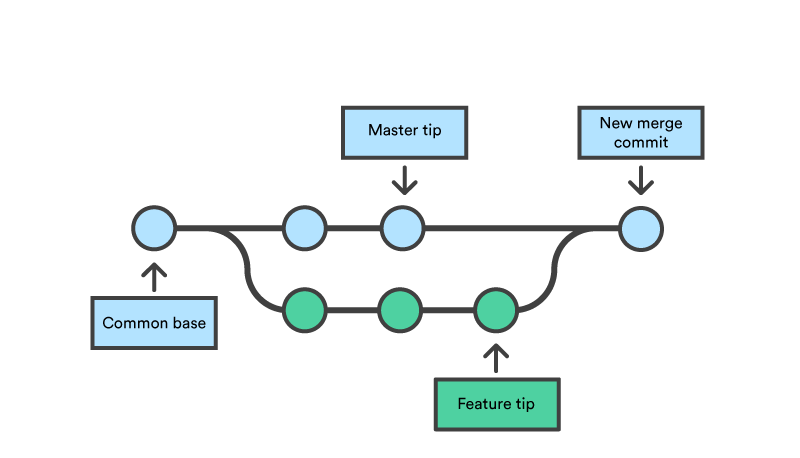
\includegraphics[width=.8\linewidth]{figs/git-branch}
\end{center}
\end{frame}


\section{Blocos}


\begin{frame}{Blocos}
	\begin{block}{Esse é um bloco}
    \begin{itemize}
        \item Isso é um teste
        \item Isso é um outro teste
    \end{itemize}
	\end{block}

	\begin{block}{}
	    Esse slide tem animação gerada pelo comando \texttt{pause}
	\end{block}

    \pause

	\begin{alertblock}{Alerta}
        Esse é um alerta
	\end{alertblock}

	\begin{exampleblock}{Bloco para exemplo}
        Exemplo com \textcolor{red}{cor em vermelho}.
    \end{exampleblock}

\end{frame}




\end{document}